\documentclass[uplatex,dvipdfmx,a4paper,11pt]{jsarticle}

\usepackage[top=25mm,bottom=25mm,left=25mm,right=25mm]{geometry}
\usepackage{array}
\usepackage{tabularx}
\usepackage{booktabs}
\usepackage{enumitem}
\usepackage{graphicx}
\usepackage{titlesec}
\usepackage[ipaex]{pxchfon}

\setlength{\parindent}{0pt}
\setlength{\parskip}{0.6em}
\titleformat{\section}
  {\normalfont\Large\bfseries}{\thesection.}{0.6em}{}
\titleformat{\subsection}
  {\normalfont\large\bfseries}{\thesubsection}{0.6em}{}
\titlespacing*{\section}{0pt}{1.2em}{0.6em}
\titlespacing*{\subsection}{0pt}{1.0em}{0.4em}

\newcommand{\sectionrule}{\par\medskip\noindent\rule{\linewidth}{0.6pt}\par\medskip}
\renewcommand{\labelitemi}{\textbullet}
\renewcommand{\labelitemii}{\textopenbullet}
\setlist[itemize]{leftmargin=1.6em,itemsep=0.1em,topsep=0.2em}
\setlist[enumerate]{leftmargin=2.0em,itemsep=0.1em,topsep=0.2em}
\providecommand{\textopenbullet}{\ensuremath{\circ}}
\begin{document}

{\LARGE\bfseries 作業ログ}\par\bigskip

報告者：齋藤　翔太\\
報告日：2026年6月30日\\
プロジェクト名：タクトーン〜IMUジェスチャーで奏でるArduinoオーケストラ〜

\sectionrule

\section{進捗サマリー（要約）}

\begin{itemize}
  \item 今回の作業進捗率：99\%
  \item マイルストーン達成状況：音量調整版スケッチを作成し，発表前確認に使える状態に整理した．
  \item 主要成果：
    \begin{itemize}
      \item {}前回作成した4声輪唱確認用スケッチをもとに，今回の修正版スケッチを作成した．
      \item {}全体音量と各パート音量を見直し，金管4声とドラムが聞き取りやすいバランスに調整した．
      \item {}ドラムを4分の4拍子として整理し，1・3拍目をキック，2・4拍目をスネアにした．
      \item {}金管の立ち上がりを速くし，ドラムとの聴感上のズレを減らした．
    \end{itemize}
  \item 重大課題（影響度：高）：なし．ただし，実機または発表環境での最終的な音量確認は継続する．
\end{itemize}

\sectionrule

\section{作業ログ（詳細トラッキング）}

{\footnotesize
\renewcommand{\arraystretch}{1.25}
\begin{tabularx}{\linewidth}{@{}>{\raggedright\arraybackslash}p{35mm}>{\raggedright\arraybackslash}p{16mm}>{\raggedright\arraybackslash}p{16mm}>{\raggedright\arraybackslash}p{15mm}>{\raggedright\arraybackslash}p{12mm}X@{}}
\hline
作業項目 & 開始日 & 完了日 & 状態 & 進捗率 & コメント \\
\hline
前回スケッチの確認と今回の調整方針整理
  & 6/24 & 6/24 & 完了 & 100\%
  & 音量，ドラムパターン，金管の立ち上がりを調整対象として整理した．\\
ドラムパターンと金管立ち上がりの調整
  & 6/27 & 6/27 & 完了 & 100\%
  & 4分の4拍子のドラムに整理し，金管の\texttt{attackSec}を短縮してズレ感を減らした．\\
\hline
\end{tabularx}
}

\sectionrule

\section{担当箇所のGC}

今回の作業内容に対応する簡易GCを図\ref{fig:saito-gc-current}に示す．
日ごとの作業内容に合わせ，前回スケッチの確認とドラム・金管調整の作業日を整理した．

\begin{figure}[htbp]
  \centering
  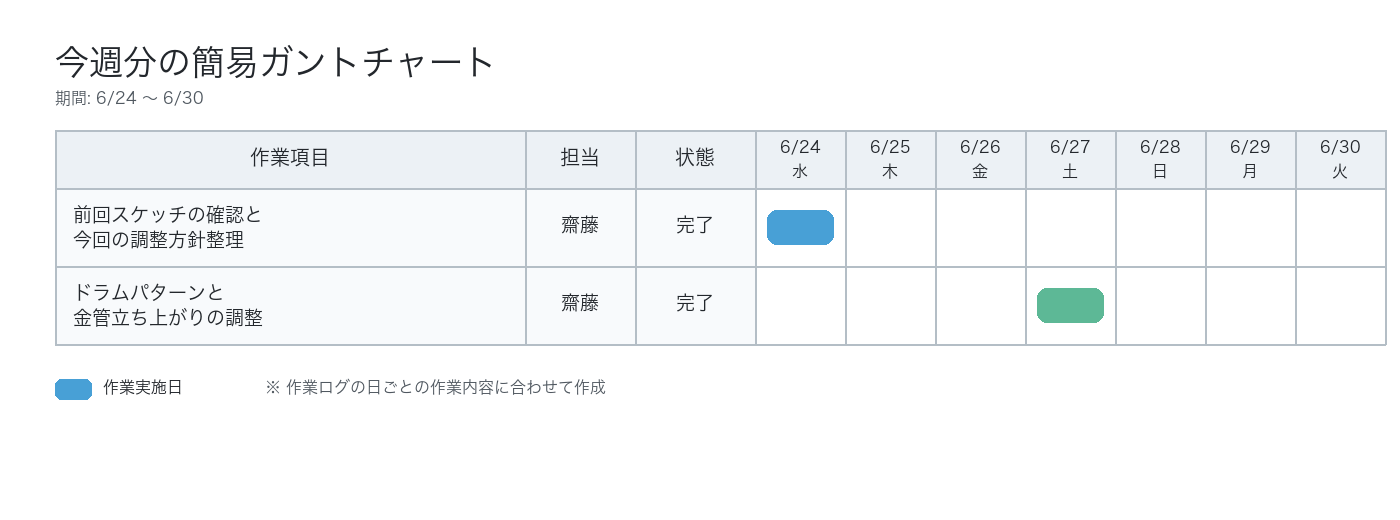
\includegraphics[width=\linewidth]{Figs/GC.png}
  \caption{今週分の簡易GC}
  \label{fig:saito-gc-current}
\end{figure}

\sectionrule

\section{日ごとの作業時間・作業内容}

{\footnotesize
\renewcommand{\arraystretch}{1.25}
\begin{tabularx}{\linewidth}{@{}>{\raggedright\arraybackslash}p{18mm}>{\raggedright\arraybackslash}p{24mm}XX@{}}
\hline
日付 & 作業時間 & 作業内容 & 成果・残課題 \\
\hline
6/24 & 1時間 & 前回スケッチの確認と今回の調整方針整理 & 音量，ドラムパターン，金管の立ち上がりを調整対象として整理した．\\
6/27 & 1時間 & ドラムパターンと金管立ち上がりの調整 & 4分の4拍子のドラムに整理し，金管の\texttt{attackSec}を短縮してズレ感を減らした．\\
\hline
\end{tabularx}
}

\sectionrule

\section{課題管理}

{\footnotesize
\renewcommand{\arraystretch}{1.25}
\begin{tabularx}{\linewidth}{@{}>{\raggedright\arraybackslash}p{30mm}X>{\raggedright\arraybackslash}p{15mm}>{\raggedright\arraybackslash}p{15mm}X@{}}
\hline
課題 & 発生原因 & 影響度 & 状態 & 対策 \\
\hline
発表環境での最終音量確認
  & Processing上の調整は完了したが，教室やスピーカー環境では聞こえ方が変わる可能性がある．
  & 中 & 継続
  & 発表前に全パートを通して再生し，必要に応じて\texttt{MASTER\_GAIN}や各パート音量を微調整する．\\
\hline
\end{tabularx}
}

\sectionrule

\section{AI利用状況と検証（再現性重視）}

\subsection{利用内容}

\begin{itemize}
  \item 利用目的：今回のスケッチの調整方針，音量バランス，ドラムパターン整理，Processing実装の補助．
  \item 入力（プロンプト要旨）：
    \begin{itemize}
      \item {}前回作成した4声輪唱スケッチをもとに，音量を聞き取りやすく調整するよう依頼した．
      \item {}ドラムを4分の4拍子として分かりやすく整理し，声部の入りと最後を強調するよう依頼した．
      \item {}金管とドラムの聴感上のズレを減らすため，拍位置を変えずに立ち上がりを調整する方法を相談した．
      \item {}今回のスケッチを単体で動作確認できるよう，音色JSONの配置とREADMEの整理を依頼した．
    \end{itemize}
  \item 出力概要：全体音量倍率，各パート音量，4分の4拍子ドラム，金管の\texttt{BRASS\_ATTACK\_SCALE}，音色JSONを同梱する構成が提示された．
\end{itemize}

\sectionrule

\subsection{検証方法}

\begin{itemize}
  \item 検証手法：AIの出力をそのまま採用せず，リポジトリ内のスケッチ，README，音色JSONを照合した．
  \item 検証手順：
    \begin{enumerate}
      \item {}Processingスケッチの定数と\texttt{PartDefinition}を確認した．
      \item {}4声の開始拍が0，8，16，24拍であり，チューバがC2相当で鳴る設定であることを確認した．
      \item {}ドラムが56拍で，1・3拍目キック，2・4拍目スネアの構成であることを確認した．
      \item {}\texttt{data/}フォルダに音色JSON 8ファイルが同梱されていることを確認した．
      \item {}READMEに実行方法と変更点が整理されていることを確認した．
    \end{enumerate}
\end{itemize}

\sectionrule

\subsection{ファクトチェック結果}

\begin{itemize}
  \item 一致点：\texttt{MASTER\_GAIN = 1.35}，\texttt{DRUM\_AMPLITUDE = 0.11}，\texttt{BRASS\_ATTACK\_SCALE = 0.45}が修正版スケッチに反映されていることを確認した．
  \item 未実施項目：発表会場のスピーカーを使った最終音量確認は未実施である．
  \item 最終判断：Processing確認用スケッチを今回の成果として記載し，環境依存の音量確認は次回の課題として扱う．
\end{itemize}

\sectionrule

\section{次回計画}

\begin{itemize}
  \item 目標：発表前に修正版スケッチを通しで再生し，発表環境での聞こえ方を確認する．
  \item 達成基準：金管4声，チューバ，ドラムが極端に埋もれたり音割れしたりしないことを確認する．
  \item 次の作業：必要に応じて，\texttt{MASTER\_GAIN}，各パートの\texttt{amplitude}，\texttt{DRUM\_AMPLITUDE}を微調整する．
  \item 将来の作業：Arduino側の楽譜データへ反映する必要が生じた場合は，実機での動作確認を行う．
\end{itemize}

\sectionrule

\section{付録}

\begin{itemize}
  \item 添付資料：
    \begin{itemize}
      \item ソースコード：\texttt{https://github.com/takushio2525/2026-hackathon-team23}
    \end{itemize}
  \item 添付範囲：
    \begin{itemize}
      \item 今回の確認対象であるProcessingスケッチ，音色JSON，READMEの全体
    \end{itemize}
\end{itemize}

\end{document}
